\documentclass[12pt,a4paper]{article}

% ─── Packages ────────────────────────────────────────────────────────
\usepackage[utf8]{inputenc}
\usepackage[T1]{fontenc}
\usepackage[english]{babel}
\usepackage{amsmath,amssymb,amsfonts}
\usepackage{graphicx}
\usepackage[margin=25mm]{geometry}
\usepackage{booktabs}
\usepackage{caption}
\usepackage{subcaption}
\usepackage{hyperref}
\usepackage{cleveref}
\usepackage{algorithm}
\usepackage{algpseudocode}
\usepackage{enumitem}
\usepackage{float}
\usepackage{tabularx}
\usepackage{xcolor}
\usepackage{natbib}
\usepackage{setspace}
\usepackage{parskip}

\onehalfspacing

\hypersetup{
    colorlinks=true,
    linkcolor=blue!60!black,
    citecolor=blue!60!black,
    urlcolor=blue!60!black,
}

% ─── Title page ──────────────────────────────────────────────────────
\begin{document}

\begin{titlepage}
\centering
\vspace*{2cm}

{\Large\textsc{KTH Royal Institute of Technology}}\\
\vspace{0.3cm}
{\large School of Electrical Engineering and Computer Science}\\
\vspace{0.3cm}
{\normalsize Degree Project in Computer Science, First Cycle}\\
\vspace{0.3cm}
{\normalsize DD143X, 15 ECTS}

\vspace{2.5cm}

{\huge\bfseries Adversarial Attacks on Cooperative\\[0.3cm] Multi-Agent Reinforcement\\[0.3cm] Learning Systems}

\vspace{2cm}

{\Large [Student Name]}

\vspace{1.5cm}

{\large Supervisors: NN}\\
\vspace{0.3cm}
{\large Examiner: [Examiner Name]}

\vspace{\fill}

{\large Stockholm, Sweden, March 2026}
\end{titlepage}

% ─── Abstract ────────────────────────────────────────────────────────
\newpage
\section*{Abstract}

Cooperative multi-agent reinforcement learning (c-MARL) enables teams of autonomous agents to solve complex tasks through collaboration. However, the robustness of these systems against adversarial attacks remains poorly understood. In this work, we systematically investigate the vulnerability of c-MARL systems to two categories of attacks: observation perturbation attacks (FGSM, PGD) and behavioral attacks (adversarial agent replacement). We train cooperative agents using MAPPO, QMIX, and a communication-enhanced CommNet architecture on the Simple Spread environment, and evaluate their resilience under various attack scenarios.

Our contributions are threefold. First, we introduce a \emph{stealth adversarial agent} that balances attack effectiveness with undetectability by constraining the KL divergence between its policy and the cooperative policy, revealing a clear trade-off between damage and detectability. Second, we conduct an exploratory cross-algorithm transferability study of adversarial attacks between MAPPO and QMIX, finding limited transfer in both observation perturbation and behavioral attacks. Third, we show that communication between agents (CommNet) paradoxically increases vulnerability to small observation perturbations, as adversarial noise propagates through the communication channel. We additionally evaluate defensive strategies---FGSM adversarial training, noise augmentation, and observation smoothing---finding that temporal observation smoothing provides the most practical defense.

\textbf{Keywords:} Multi-agent reinforcement learning, adversarial attacks, cooperative AI, robustness, stealth attacks

\newpage
\section*{Sammanfattning}

Kooperativ multiagent-f{\"o}rst{\"a}rkningsinl{\"a}rning (c-MARL) m{\"o}jligg{\"o}r att team av autonoma agenter l{\"o}ser komplexa uppgifter genom samarbete. Robustheten hos dessa system mot fientliga attacker {\"a}r dock d{\aa}ligt f{\"o}rst{\aa}dd. I detta arbete unders{\"o}ker vi systematiskt s{\aa}rbarheten hos c-MARL-system mot tv{\aa} kategorier av attacker: observationsperturbationsattacker (FGSM, PGD) och beteendeattacker (byte av agent mot en fientlig agent). Vi tr{\"a}nar kooperativa agenter med MAPPO, QMIX och en kommunikationsf{\"o}rst{\"a}rkt CommNet-arkitektur i milj{\"o}n Simple Spread, och utv{\"a}rderar deras motst{\aa}ndskraft under olika attackscenarier.

V{\aa}ra bidrag {\"a}r trefaldiga. F{\"o}rst introducerar vi en \emph{stealth-attackagent} som balanserar attackeffektivitet med odetekterbarhet genom att begr{\"a}nsa KL-divergensen mellan dess policy och den kooperativa policyn, vilket avsl{\"o}jar en tydlig avv{\"a}gning mellan skada och detekterbarhet. F{\"o}r det andra genomf{\"o}r vi en utforskande {\"o}verf{\"o}rbarhetsstudie av attacker mellan MAPPO och QMIX, och finner begr{\"a}nsad {\"o}verf{\"o}rbarhet. F{\"o}r det tredje visar vi att kommunikation mellan agenter (CommNet) paradoxalt nog {\"o}kar s{\aa}rbarheten f{\"o}r sm{\aa} observationsperturbationer, d{\aa} fientligt brus propagerar genom kommunikationskanalen. Vi utv{\"a}rderar {\"a}ven motmedel --- FGSM-baserad fientlig tr{\"a}ning, brusaugmentering och observationsutj{\"a}mning --- och finner att temporal observationsutj{\"a}mning ger det mest praktiska f{\"o}rsvaret.

\newpage
\tableofcontents
\newpage

% ═════════════════════════════════════════════════════════════════════
% CHAPTER 1: INTRODUCTION
% ═════════════════════════════════════════════════════════════════════
\section{Introduction}
\label{sec:intro}

Multi-agent reinforcement learning (MARL) has emerged as a powerful paradigm for training autonomous agents to coordinate and cooperate in complex environments \citep{busoniu2008comprehensive}. In cooperative MARL (c-MARL), a team of agents jointly optimizes a shared objective, finding applications in autonomous driving \citep{wang2025robust}, search-and-rescue operations, robotic swarm coordination, and network management \citep{kazari2023decentralized}. As these systems move from simulation to real-world deployment, understanding their failure modes becomes critical.

Adversarial machine learning has revealed that deep learning systems are surprisingly brittle. In single-agent RL, small perturbations to an agent's observations can cause catastrophic policy failures \citep{huang2017adversarial}. The multi-agent setting introduces additional attack surfaces: an adversary may corrupt one or more agents' observations, compromise communication channels, or even replace a cooperative agent with a malicious one. The complex interactions between agents mean that attacking a single agent can cascade through the entire team.

Despite growing interest, several key questions remain unanswered:

\begin{enumerate}[label=(\roman*)]
    \item How effective are standard adversarial attacks (FGSM, PGD) against c-MARL systems, and how do they scale with perturbation magnitude?
    \item Are behavioral attacks (adversarial agent replacement) more effective than observation perturbation?
    \item Do adversarial attacks transfer across different c-MARL algorithms?
    \item Does inter-agent communication increase or decrease robustness?
    \item Can an adversarial agent cause significant damage while remaining undetected?
\end{enumerate}

\subsection{Contributions}

This thesis makes the following contributions:

\begin{enumerate}
    \item \textbf{Systematic attack taxonomy and evaluation.} We implement and compare observation perturbation attacks (FGSM, iterative FGSM/PGD, random noise) and behavioral attacks (trained adversarial agent) against MAPPO-trained cooperative agents, providing a comprehensive robustness profile.

    \item \textbf{Stealth adversarial agents.} We propose a KL-divergence-constrained adversarial agent that balances attack effectiveness with undetectability. By varying the constraint threshold, we map the Pareto frontier of the damage--detectability trade-off.

    \item \textbf{Cross-algorithm transferability (exploratory).} We evaluate whether attacks crafted against one c-MARL algorithm (MAPPO) transfer to a fundamentally different algorithm (QMIX). While our QMIX baseline did not fully converge---a known challenge for value decomposition methods on this task---the results suggest limited transferability and motivate further study with better-matched baselines.

    \item \textbf{Communication as a vulnerability.} We compare standard MAPPO (no communication) with CommNet under identical attacks, demonstrating that learned communication channels propagate adversarial noise and increase vulnerability at low perturbation magnitudes.

    \item \textbf{Countermeasure evaluation.} We evaluate FGSM adversarial training, noise augmentation, and observation smoothing as defensive strategies, and additionally test adaptive attacks that account for the defense mechanism.
\end{enumerate}

\subsection{Outline}

The remainder of this thesis is organized as follows. \Cref{sec:background} provides the theoretical background on reinforcement learning, multi-agent RL, and adversarial attacks. \Cref{sec:related} surveys related work. \Cref{sec:method} describes the environment, algorithms, attack strategies, and countermeasures we implement. \Cref{sec:experiments} details the experimental setup. \Cref{sec:results} presents the results. \Cref{sec:discussion} discusses the findings, limitations, and implications. \Cref{sec:conclusion} concludes the thesis with directions for future work.

% ═════════════════════════════════════════════════════════════════════
% CHAPTER 2: BACKGROUND
% ═════════════════════════════════════════════════════════════════════
\section{Background}
\label{sec:background}

\subsection{Reinforcement Learning}

Reinforcement learning (RL) formalizes sequential decision-making as a Markov Decision Process (MDP). An MDP is defined by a tuple $(\mathcal{S}, \mathcal{A}, P, R, \gamma)$, where $\mathcal{S}$ is the state space, $\mathcal{A}$ is the action space, $P(s' | s, a)$ is the transition function, $R(s, a)$ is the reward function, and $\gamma \in [0, 1)$ is the discount factor. An agent follows a policy $\pi(a | s)$ that maps states to action distributions, aiming to maximize the expected discounted return:
\begin{equation}
    J(\pi) = \mathbb{E}_\pi \left[ \sum_{t=0}^{\infty} \gamma^t R(s_t, a_t) \right].
\end{equation}

\subsubsection{Policy Gradient Methods}

Policy gradient methods directly optimize the policy by estimating the gradient of $J(\pi)$ with respect to the policy parameters $\theta$. The REINFORCE estimator \citep{williams1992simple} gives:
\begin{equation}
    \nabla_\theta J(\theta) = \mathbb{E}_\pi \left[ \nabla_\theta \log \pi_\theta(a_t | s_t) \cdot A_t \right],
\end{equation}
where $A_t$ is the advantage function. Proximal Policy Optimization (PPO) \citep{schulman2017proximal} stabilizes training by constraining the policy update with a clipped surrogate objective:
\begin{equation}
    L^{\text{CLIP}}(\theta) = \mathbb{E}_t \left[ \min\left( r_t(\theta) A_t, \; \text{clip}(r_t(\theta), 1 - \epsilon, 1 + \epsilon) A_t \right) \right],
    \label{eq:ppo}
\end{equation}
where $r_t(\theta) = \pi_\theta(a_t | s_t) / \pi_{\theta_\text{old}}(a_t | s_t)$ is the importance sampling ratio.

\subsubsection{Value Decomposition}

An alternative to policy gradient methods is value-based learning, where the agent learns a Q-function $Q(s, a) = \mathbb{E}_\pi[\sum_{t=0}^\infty \gamma^t R_t | s_0 = s, a_0 = a]$ and acts greedily with respect to it.

\subsection{Multi-Agent Reinforcement Learning}

In multi-agent settings, the environment is modeled as a Decentralized Partially Observable Markov Decision Process (Dec-POMDP), defined by $(\mathcal{N}, \mathcal{S}, \{\mathcal{A}_i\}, \{\mathcal{O}_i\}, P, R, \gamma)$, where $\mathcal{N}$ is the set of $n$ agents, $\mathcal{O}_i$ is the observation space of agent $i$, and each agent $i$ receives a local observation $o_i$ that provides only partial information about the global state $s$.

The \emph{centralized training with decentralized execution} (CTDE) paradigm \citep{oliehoek2008optimal} addresses this by allowing access to global information during training while requiring agents to act based only on local observations at execution time.

\subsubsection{MAPPO}

Multi-Agent PPO (MAPPO) \citep{yu2022surprising} applies PPO to multi-agent settings under the CTDE paradigm. Each agent $i$ has a decentralized actor $\pi_{\theta_i}(a_i | o_i)$ that outputs actions based on local observations. A centralized critic $V_\phi(s)$ takes the global state $s$ (e.g., the concatenation of all agents' observations) and estimates the team value function. All agents share the PPO clipped objective (\cref{eq:ppo}) with a shared team reward. In our implementation, agents share actor parameters, which improves sample efficiency and enforces behavioral symmetry.

\subsubsection{QMIX}

QMIX \citep{rashid2018qmix} uses value decomposition to factorize the joint action-value function into per-agent utilities. Each agent $i$ learns an individual Q-function $Q_i(o_i, a_i)$, and a mixing network combines these into a joint value:
\begin{equation}
    Q_\text{tot}(\mathbf{o}, \mathbf{a}, s) = f_\text{mix}(Q_1(o_1, a_1), \ldots, Q_n(o_n, a_n); s),
\end{equation}
where $f_\text{mix}$ is a feed-forward network with non-negative weights (generated by hypernetworks conditioned on the global state $s$). The non-negativity constraint ensures monotonicity:
\begin{equation}
    \frac{\partial Q_\text{tot}}{\partial Q_i} \geq 0, \quad \forall i,
\end{equation}
meaning that the joint greedy action equals the collection of individually greedy actions. This enables decentralized execution while training with the richer global signal.

\subsubsection{CommNet}

CommNet \citep{sukhbaatar2016learning} extends multi-agent architectures with learned communication. Agents exchange continuous message vectors over multiple communication rounds. At each round $k$, agent $i$ computes a message $m_i^k$ from its hidden state and receives the mean of other agents' messages:
\begin{equation}
    h_i^{k+1} = \sigma\left(W^k \left[h_i^k \;;\; \frac{1}{n-1}\sum_{j \neq i} m_j^k\right]\right),
\end{equation}
where $[\ ;\ ]$ denotes concatenation and $\sigma$ is a nonlinearity. This allows agents to coordinate their actions based on shared information. We integrate CommNet as the actor in a MAPPO-style training framework.

\subsection{Adversarial Attacks on Neural Networks}

\subsubsection{Fast Gradient Sign Method (FGSM)}

FGSM \citep{goodfellow2015explaining} generates adversarial perturbations by taking a single gradient step in the direction that maximizes the loss:
\begin{equation}
    x_\text{adv} = x + \epsilon \cdot \text{sign}\left(\nabla_x \mathcal{L}(\theta, x, y)\right),
\end{equation}
where $\epsilon$ controls the perturbation magnitude. In our c-MARL setting, we perturb an agent's observation $o_i$ to decrease the log-probability of the greedy action:
\begin{equation}
    o_i^\text{adv} = o_i - \epsilon \cdot \text{sign}\left(\nabla_{o_i} \log \pi_\theta(a^*_i | o_i)\right),
    \label{eq:fgsm_attack}
\end{equation}
where $a^*_i = \arg\max_a \pi_\theta(a | o_i)$.

\subsubsection{Projected Gradient Descent (PGD)}

PGD \citep{madry2018towards} extends FGSM to an iterative attack, taking multiple smaller gradient steps and projecting back into the $\epsilon$-ball after each step:
\begin{equation}
    o_i^{t+1} = \Pi_\epsilon \left( o_i^t - \alpha \cdot \text{sign}\left(\nabla_{o_i^t} \log \pi_\theta(a^*_i | o_i^t) \right) \right),
\end{equation}
where $\Pi_\epsilon$ projects onto the $\ell_\infty$-ball of radius $\epsilon$ around the clean observation.

% ═════════════════════════════════════════════════════════════════════
% CHAPTER 3: RELATED WORK
% ═════════════════════════════════════════════════════════════════════
\section{Related Work}
\label{sec:related}

\subsection{Adversarial Attacks on Single-Agent RL}

\citet{huang2017adversarial} first demonstrated that deep RL policies are vulnerable to adversarial perturbations, showing that FGSM attacks on Atari game observations can cause significant performance degradation. \citet{pinto2017robust} proposed Robust Adversarial RL (RARL), training an adversary jointly with the protagonist to improve robustness. These works established the foundation for studying adversarial robustness in RL.

\subsection{Adversarial Attacks on Cooperative MARL}

\citet{lin2020robustness} provided the first systematic study of adversarial attacks on cooperative MARL, showing that perturbing a single agent's observations can degrade the entire team's performance. They evaluated observation perturbation attacks on several c-MARL benchmarks. \citet{guo2022towards} extended this with comprehensive testing frameworks for c-MARL robustness.

The c-MBA method \citep{wu2022cmba} introduced model-based adversarial attacks that learn environment dynamics to craft more effective perturbations. More recently, \citet{li2025ami} proposed Adversarial Minority Influence (AMI), a black-box attack enabling a single adversarial agent to mislead the majority into worst-case cooperation. AMI achieves this through a unilateral influence filter and targeted adversarial oracle, demonstrating attacks on robot swarms and StarCraft~II.

\citet{standen2025acm} presented a comprehensive survey of adversarial attacks and defenses in MARL, categorizing attacks into observation perturbation, action perturbation, and communication perturbation.

\subsection{Stealth and Constrained Attacks}

The idea of constraining adversarial behavior for undetectability has been explored in cyber-physical systems \citep{kung2017optimal}, where KL divergence is used to bound the statistical deviation of attack signals. In the MARL context, recent work \citep{andam2025constrained} has studied constrained black-box attacks, demonstrating that an adversary with limited information can still inflict significant damage. Our stealth adversarial agent differs by explicitly training the adversary with a KL-divergence constraint against the cooperative policy.

\subsection{Defenses and Robustness}

Adversarial training \citep{madry2018towards} remains the most common defense, training models on adversarially perturbed inputs. In the MARL setting, \citet{wang2025robust} proposed robust constrained cooperative MARL for self-driving vehicles. Anomaly detection approaches \citep{kazari2023decentralized} have been proposed to detect adversarial agents based on deviations from expected behavior.

% ═════════════════════════════════════════════════════════════════════
% CHAPTER 4: METHOD
% ═════════════════════════════════════════════════════════════════════
\section{Method}
\label{sec:method}

\subsection{Environment: Simple Spread}

We use the Simple Spread environment from the Multi-Agent Particle Environment (MPE) \citep{lowe2017multi}, accessed through the PettingZoo library \citep{terry2021pettingzoo}. In this task, $n$ agents must navigate to cover $n$ landmarks while avoiding collisions. The team reward has two components: (i)~the negative sum of minimum distances from each landmark to the nearest agent, incentivizing full coverage, and (ii)~a collision penalty applied when agents overlap, discouraging clustering. The environment parameter \texttt{local\_ratio=0.5} (default) determines the mix of local vs.\ global reward.

Each agent receives an 18-dimensional observation (for $n=3$) consisting of: its own velocity (2D), its own position (2D), relative positions of all $n=3$ landmarks ($3 \times 2 = 6$D), relative positions of the other $n-1=2$ agents ($2 \times 2 = 4$D), and communication signals from the other agents ($2 \times 2 = 4$D). Communication values are zero unless agents have a learned communication channel. The action space is discrete with 5 actions: no-op, left, right, down, up.

\subsection{Cooperative Algorithms}

We implement three cooperative algorithms:

\textbf{MAPPO} with shared actor parameters, a centralized critic taking the concatenated observations as global state, hidden dimension 128, and PPO hyperparameters: $\gamma = 0.99$, $\lambda_\text{GAE} = 0.95$, $\epsilon_\text{clip} = 0.2$, learning rate $5 \times 10^{-4}$.

\textbf{QMIX} with per-agent Q-networks using GRU recurrence (hidden dimension 64), a mixing network with hypernetwork-generated weights (mixing dimension 32), $\epsilon$-greedy exploration decaying from 1.0 to 0.05, and experience replay buffer of size 5000.

\textbf{CommNet-MAPPO:} MAPPO with the actor replaced by a CommNet architecture using 2 communication rounds. Agents encode observations, exchange message vectors, and decode actions conditioned on received messages.

All models are trained for 20{,}000 episodes with batch updates every 10 episodes (for PPO-based methods).

\subsection{Attack Strategies}

\subsubsection{Observation Perturbation Attacks}

We implement three white-box, inference-time attacks:

\begin{enumerate}
    \item \textbf{FGSM:} Single-step gradient attack (\cref{eq:fgsm_attack}) with varying $\epsilon \in \{0.01, 0.05, 0.1, 0.2, 0.3, 0.5, 0.75, 1.0\}$.
    \item \textbf{Iterative FGSM (PGD):} 10-step iterative attack with step size $\alpha = 2\epsilon / 10$, random initialization within the $\epsilon$-ball, and projection after each step.
    \item \textbf{Random noise:} Uniform noise baseline $o_i^\text{adv} = o_i + \mathcal{U}(-\epsilon, \epsilon)$.
\end{enumerate}

\subsubsection{Behavioral Attacks: Adversarial Agent}

We replace one cooperative agent (agent 0) with a malicious agent trained to minimize the team reward. The adversarial agent is trained using PPO with the negated team reward $-R_\text{team}$ as its objective, while the remaining cooperative agents use the frozen pre-trained MAPPO policy. This creates a challenging game where the adversary must learn to exploit the cooperative agents' fixed strategies.

\subsubsection{Stealth Adversarial Agent}
\label{sec:stealth}

A key limitation of the unconstrained adversarial agent is its detectability---its behavior diverges significantly from the cooperative policy. We propose a \emph{stealth adversarial agent} that solves the constrained optimization:
\begin{equation}
    \max_{\theta_\text{adv}} \; \mathbb{E}\left[-R_\text{team}\right] \quad \text{s.t.} \quad D_\text{KL}\left(\pi_{\theta_\text{adv}} \;\|\; \pi_\text{coop}\right) \leq \delta,
\end{equation}
where $\delta$ is the stealth threshold controlling the trade-off between attack effectiveness and detectability. In practice, we train the adversary using PPO, which minimizes a policy loss $L_\text{PPO}$ derived from the negated team reward. We incorporate the KL constraint via Lagrangian relaxation, yielding the \emph{minimization} problem:
\begin{equation}
    \min_{\theta_\text{adv}} \; L_\text{PPO}(\theta_\text{adv}) + \lambda \cdot \max\left(0, \; D_\text{KL}(\pi_{\theta_\text{adv}} \| \pi_\text{coop}) - \delta\right),
\end{equation}
where $\lambda \geq 0$ is a learnable Lagrange multiplier. The penalty term increases the loss when the KL constraint is violated, discouraging the adversary from deviating too far from the cooperative policy. The multiplier $\lambda$ is updated via dual gradient ascent:
\begin{equation}
    \lambda \leftarrow \lambda + \eta_\lambda \left(D_\text{KL}(\pi_{\theta_\text{adv}} \| \pi_\text{coop}) - \delta\right),
\end{equation}
which increases $\lambda$ when the constraint is violated and decreases it when satisfied.

We train stealth adversaries with $\delta \in \{0.1, 0.5, 2.0\}$, spanning tight to loose constraints.

\subsection{Countermeasures}

\subsubsection{Noise Augmentation}

As a simple baseline defense, we retrain MAPPO with random observation perturbations injected during training: with probability 0.5, each observation is perturbed by $\mathcal{U}(-0.2, 0.2)$ before action selection. This exposes the policy to noisy observations during training, encouraging some robustness, but the perturbations are not adversarially chosen.

\subsubsection{FGSM Adversarial Training}

Following \citet{madry2018towards}, we implement true adversarial training by generating FGSM perturbations during data collection. With probability 0.5, the agent's observation is perturbed using the current policy's own gradient (as in \cref{eq:fgsm_attack}) before action selection. Unlike noise augmentation, this exposes the policy to \emph{worst-case} perturbations at each training step.

\subsubsection{Observation Smoothing}

We apply temporal exponential moving average (EMA) smoothing to observations:
\begin{equation}
    \hat{o}_i^t = \alpha \cdot o_i^t + (1 - \alpha) \cdot \hat{o}_i^{t-1},
\end{equation}
where $\alpha \in (0, 1]$ controls the smoothing strength. This attenuates sudden perturbations while preserving the observation trend. We evaluate $\alpha \in \{0.2, 0.5, 0.8\}$.

\subsubsection{Anomaly Detection}

We implement a per-step, per-agent action divergence detector that monitors each agent's behavior against the cooperative policy. For each agent $i$ at each time step $t$, we compute the negative log-probability of its taken action under the reference cooperative policy:
\begin{equation}
    d_i^t = -\log \pi_\text{coop}(a_i^t | o_i^t).
\end{equation}
An agent is flagged as anomalous at step $t$ if the windowed average $\bar{d}_i^t = \frac{1}{W}\sum_{k=t-W+1}^{t} d_i^k$ exceeds a threshold $\tau$. We use window size $W=5$ and $\tau = 2.0$, chosen as two standard deviations above the mean $d_i^t$ observed under clean cooperative play. The reported TPR and FPR are computed per-step: TPR is the fraction of steps where the adversarial agent is correctly flagged, and FPR is the fraction of steps where a cooperative agent is incorrectly flagged.

% ═════════════════════════════════════════════════════════════════════
% CHAPTER 5: EXPERIMENTS
% ═════════════════════════════════════════════════════════════════════
\section{Experimental Setup}
\label{sec:experiments}

\subsection{Training}

All experiments use PyTorch 2.9 and PettingZoo/MPE2. The Simple Spread environment uses $n=3$ agents with discrete actions and episode length 25 steps.

\textbf{MAPPO:} 20{,}000 episodes, batch size 10 episodes, 15 PPO epochs per update, hidden dimension 128, learning rates $5 \times 10^{-4}$.

\textbf{QMIX:} 20{,}000 episodes, replay buffer size 5000, batch size 32, target network update every 200 episodes, $\epsilon$-greedy decay over 5{,}000 steps.

\textbf{CommNet:} Same as MAPPO but with CommNet actor (2 communication rounds).

\textbf{Robust MAPPO:} Same as MAPPO with adversarial training ($\epsilon = 0.2$, probability 0.5).

\textbf{Adversarial agents:} 5{,}000 episodes, trained against frozen cooperative MAPPO.

\textbf{Stealth adversarial agents:} 5{,}000 episodes each for $\delta \in \{0.1, 0.5, 2.0\}$.

\subsection{Evaluation Protocol}

All attacks are evaluated over 100 episodes with deterministic policies. We report mean team reward and standard deviation. For stealth attacks, we additionally report the true positive rate (TPR) and false positive rate (FPR) of the anomaly detector.

The baseline performance levels are:
\begin{itemize}
    \item \textbf{Random agents:} $-77.1 \pm 25.2$ (100 episodes)
    \item \textbf{Trained MAPPO:} $-65.5$ [$-69.9, -61.1$] (mean across 5 seeds, 95\% CI)
\end{itemize}

% ═════════════════════════════════════════════════════════════════════
% CHAPTER 6: RESULTS
% ═════════════════════════════════════════════════════════════════════
\section{Results}
\label{sec:results}

\subsection{Baseline Attack Evaluation}

\begin{table}[H]
\centering
\caption{Effect of observation perturbation attacks on MAPPO. Results are mean reward across 5 training seeds (100 eval episodes each) with 95\% confidence intervals. Significance tested with paired $t$-test across seeds.}
\label{tab:obs_attacks}
\begin{tabular}{llrl}
\toprule
Attack & $\epsilon$ & Mean Reward [95\% CI] & $p$-value \\
\midrule
Clean & --- & $-65.5\ [-69.9, -61.1]$ & --- \\
\midrule
Random noise & 0.5 & $-66.0\ [-69.7, -62.3]$ & n.s. \\
Random noise & 1.0 & $-67.8\ [-71.4, -64.2]$ & n.s. \\
\midrule
FGSM (all agents) & 0.1 & $-66.3\ [-69.2, -63.5]$ & n.s. \\
FGSM (all agents) & 0.2 & $-68.8\ [-71.5, -66.1]$ & --- \\
FGSM (all agents) & 0.5 & $-75.0\ [-79.6, -70.3]$ & $0.012^*$ \\
FGSM (all agents) & 1.0 & $-82.2\ [-88.0, -76.4]$ & $0.005^{**}$ \\
\midrule
PGD (all agents) & 0.5 & $-67.7\ [-71.1, -64.4]$ & n.s. \\
PGD (all agents) & 1.0 & $-68.7\ [-71.6, -65.9]$ & n.s. \\
\midrule
\textbf{Adversarial agent} & --- & $\mathbf{-97.2}$ & --- \\
\bottomrule
\end{tabular}
\end{table}

\Cref{tab:obs_attacks} reveals several findings. FGSM at $\epsilon \geq 0.5$ produces statistically significant reward degradation ($p < 0.05$), while smaller perturbations and PGD at all tested levels are not distinguishable from clean performance. The adversarial agent (single training seed) produces far greater damage than any observation perturbation.

\begin{figure}[H]
\centering
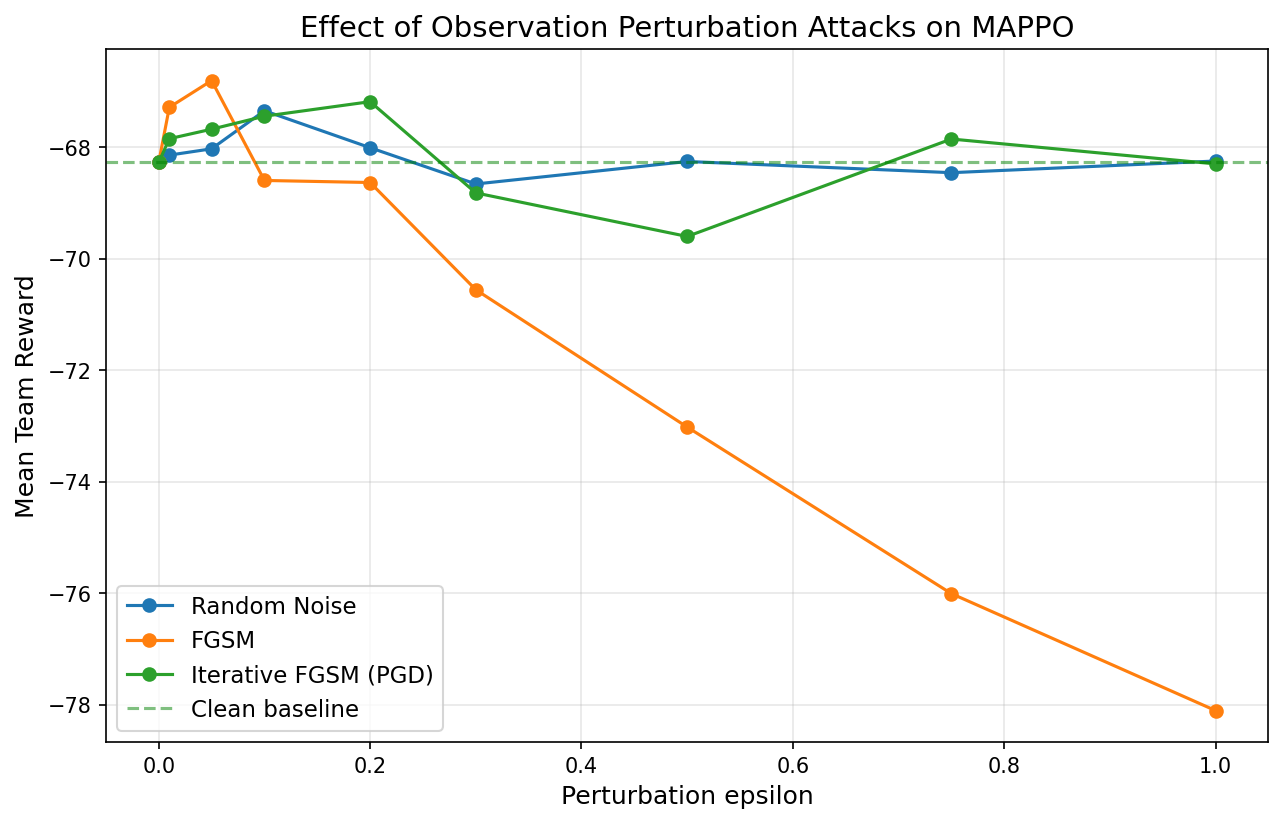
\includegraphics[width=0.85\textwidth]{figures/epsilon_sweep.png}
\caption{Mean team reward vs. perturbation $\epsilon$ for three observation attack methods. FGSM degrades reward monotonically, while PGD and random noise have limited effect.}
\label{fig:epsilon_sweep}
\end{figure}

\begin{figure}[H]
\centering
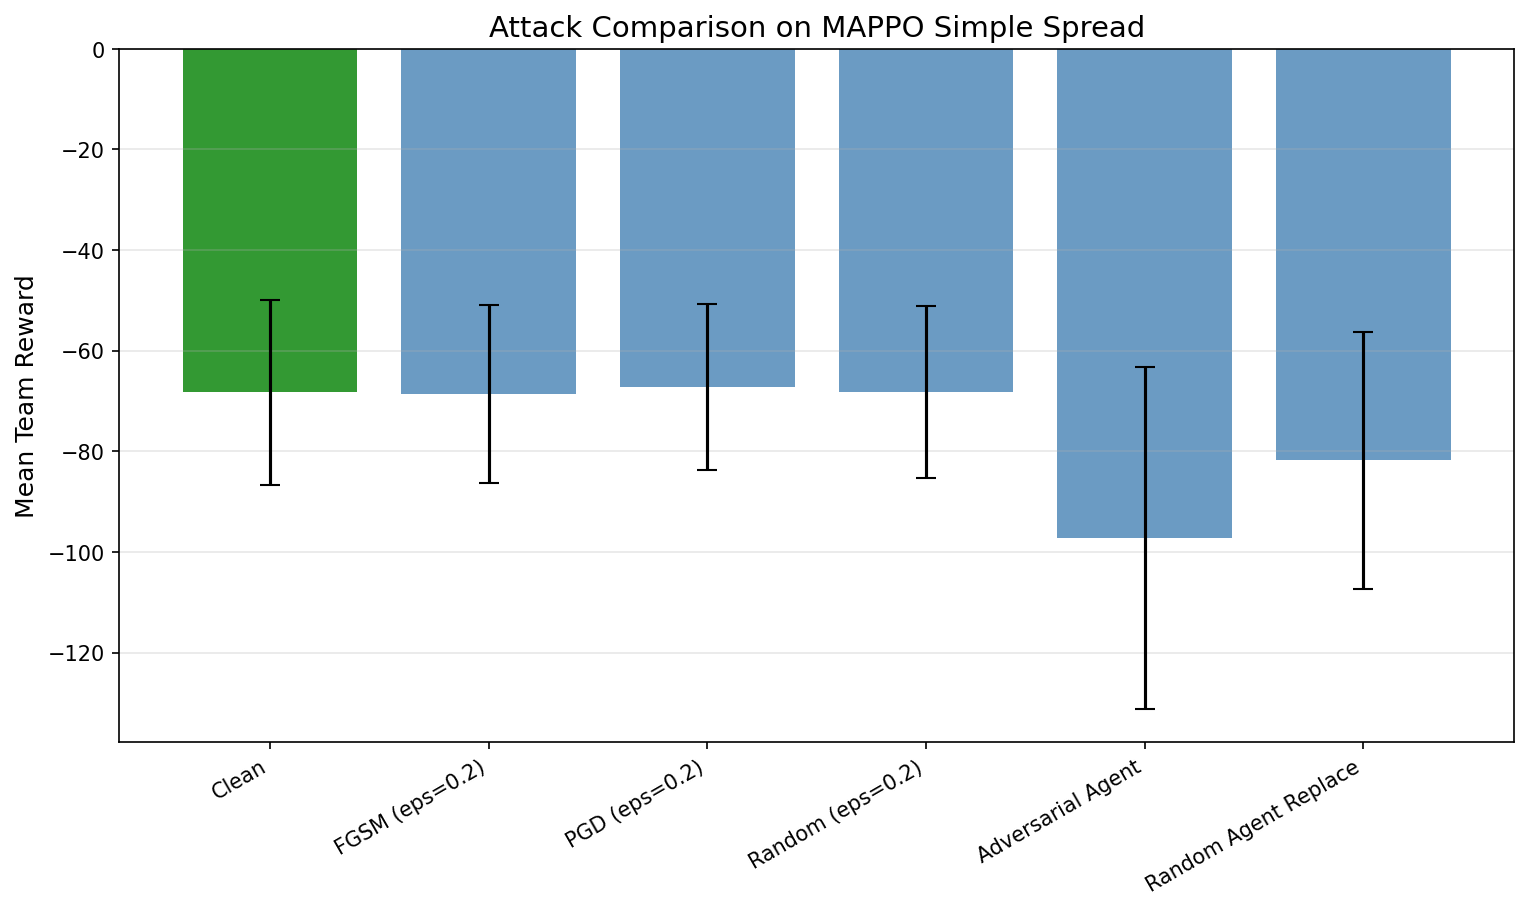
\includegraphics[width=0.85\textwidth]{figures/attack_comparison.png}
\caption{Comparison of all attack types at $\epsilon = 0.2$. The adversarial agent (behavioral attack) is dramatically more effective than any observation perturbation.}
\label{fig:attack_comparison}
\end{figure}

\subsection{Why FGSM Outperforms PGD}

The counter-intuitive finding that single-step FGSM outperforms iterative PGD deserves analysis. We hypothesize that in discrete action spaces, the objective landscape is piecewise constant---the action only changes when the perturbation crosses a decision boundary. PGD's small iterative steps may oscillate around these boundaries without crossing them.

\begin{figure}[H]
\centering
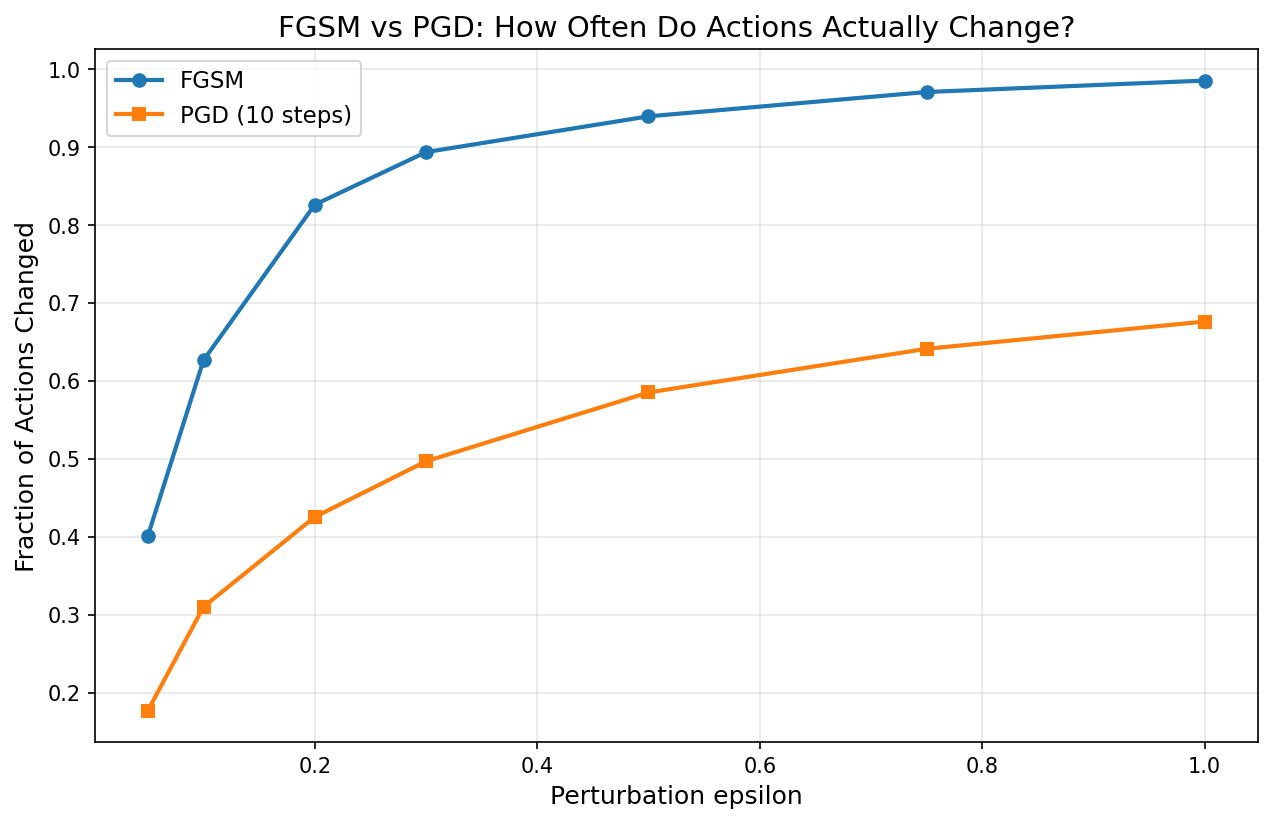
\includegraphics[width=0.8\textwidth]{figures/fgsm_vs_pgd_analysis.png}
\caption{Fraction of actions changed from the clean policy. FGSM changes actions more frequently than PGD at every $\epsilon$ level, explaining its greater effectiveness.}
\label{fig:fgsm_vs_pgd}
\end{figure}

\Cref{fig:fgsm_vs_pgd} confirms this: at $\epsilon = 0.5$, FGSM changes approximately 80\% of actions while PGD changes only 60\%. FGSM's single large step crosses more decision boundaries in the discrete action space.

We conducted a PGD ablation study varying the number of steps (3, 5, 10, 20, 50) and random initialization (on/off) across 5 training seeds. None of these variants produced reward degradation distinguishable from clean performance at $\epsilon = 0.5$ (all within $[-72.5, -62.6]$, overlapping the clean CI $[-69.9, -61.1]$). This confirms that PGD's ineffectiveness is not an artifact of our specific hyperparameter choice, but a robust phenomenon in this discrete-action setting. This finding is specific to discrete-action environments and may not generalize to continuous-action settings.

\subsection{Gradient Sensitivity Analysis}

\begin{figure}[H]
\centering
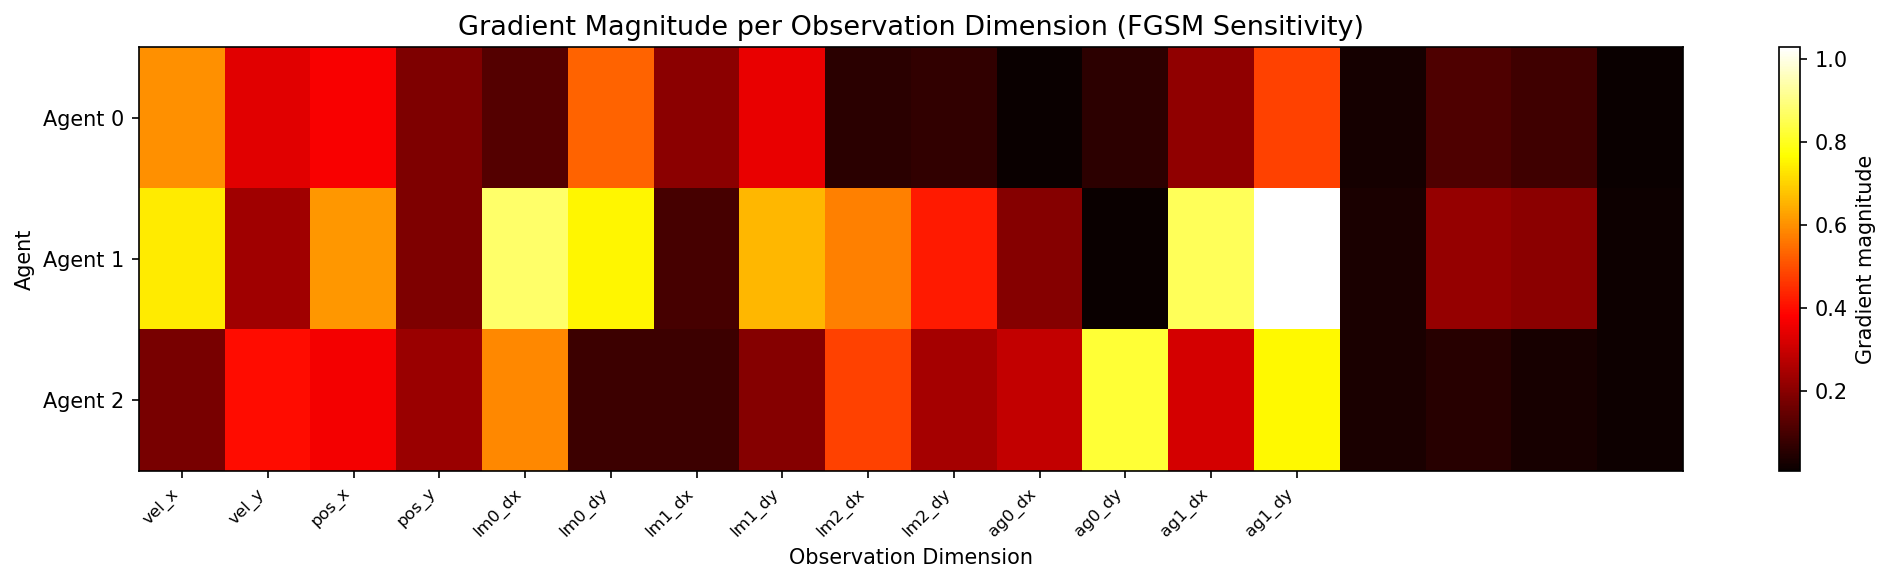
\includegraphics[width=\textwidth]{figures/gradient_heatmap.png}
\caption{FGSM gradient magnitude per observation dimension. Landmark relative positions and other-agent positions show the highest sensitivity.}
\label{fig:gradient_heatmap}
\end{figure}

\Cref{fig:gradient_heatmap} shows which observation dimensions are most sensitive to perturbation. Landmark relative positions ($\texttt{lm\_dx}, \texttt{lm\_dy}$) and other-agent positions ($\texttt{ag\_dx}, \texttt{ag\_dy}$) exhibit the largest gradients. This is intuitive: the agent's action primarily depends on where landmarks and other agents are, so perturbing these dimensions has the greatest impact on action selection. Velocity dimensions are less sensitive, suggesting the policy is more robust to kinematic noise.

\subsection{Trajectory Analysis}

\begin{figure}[H]
\centering
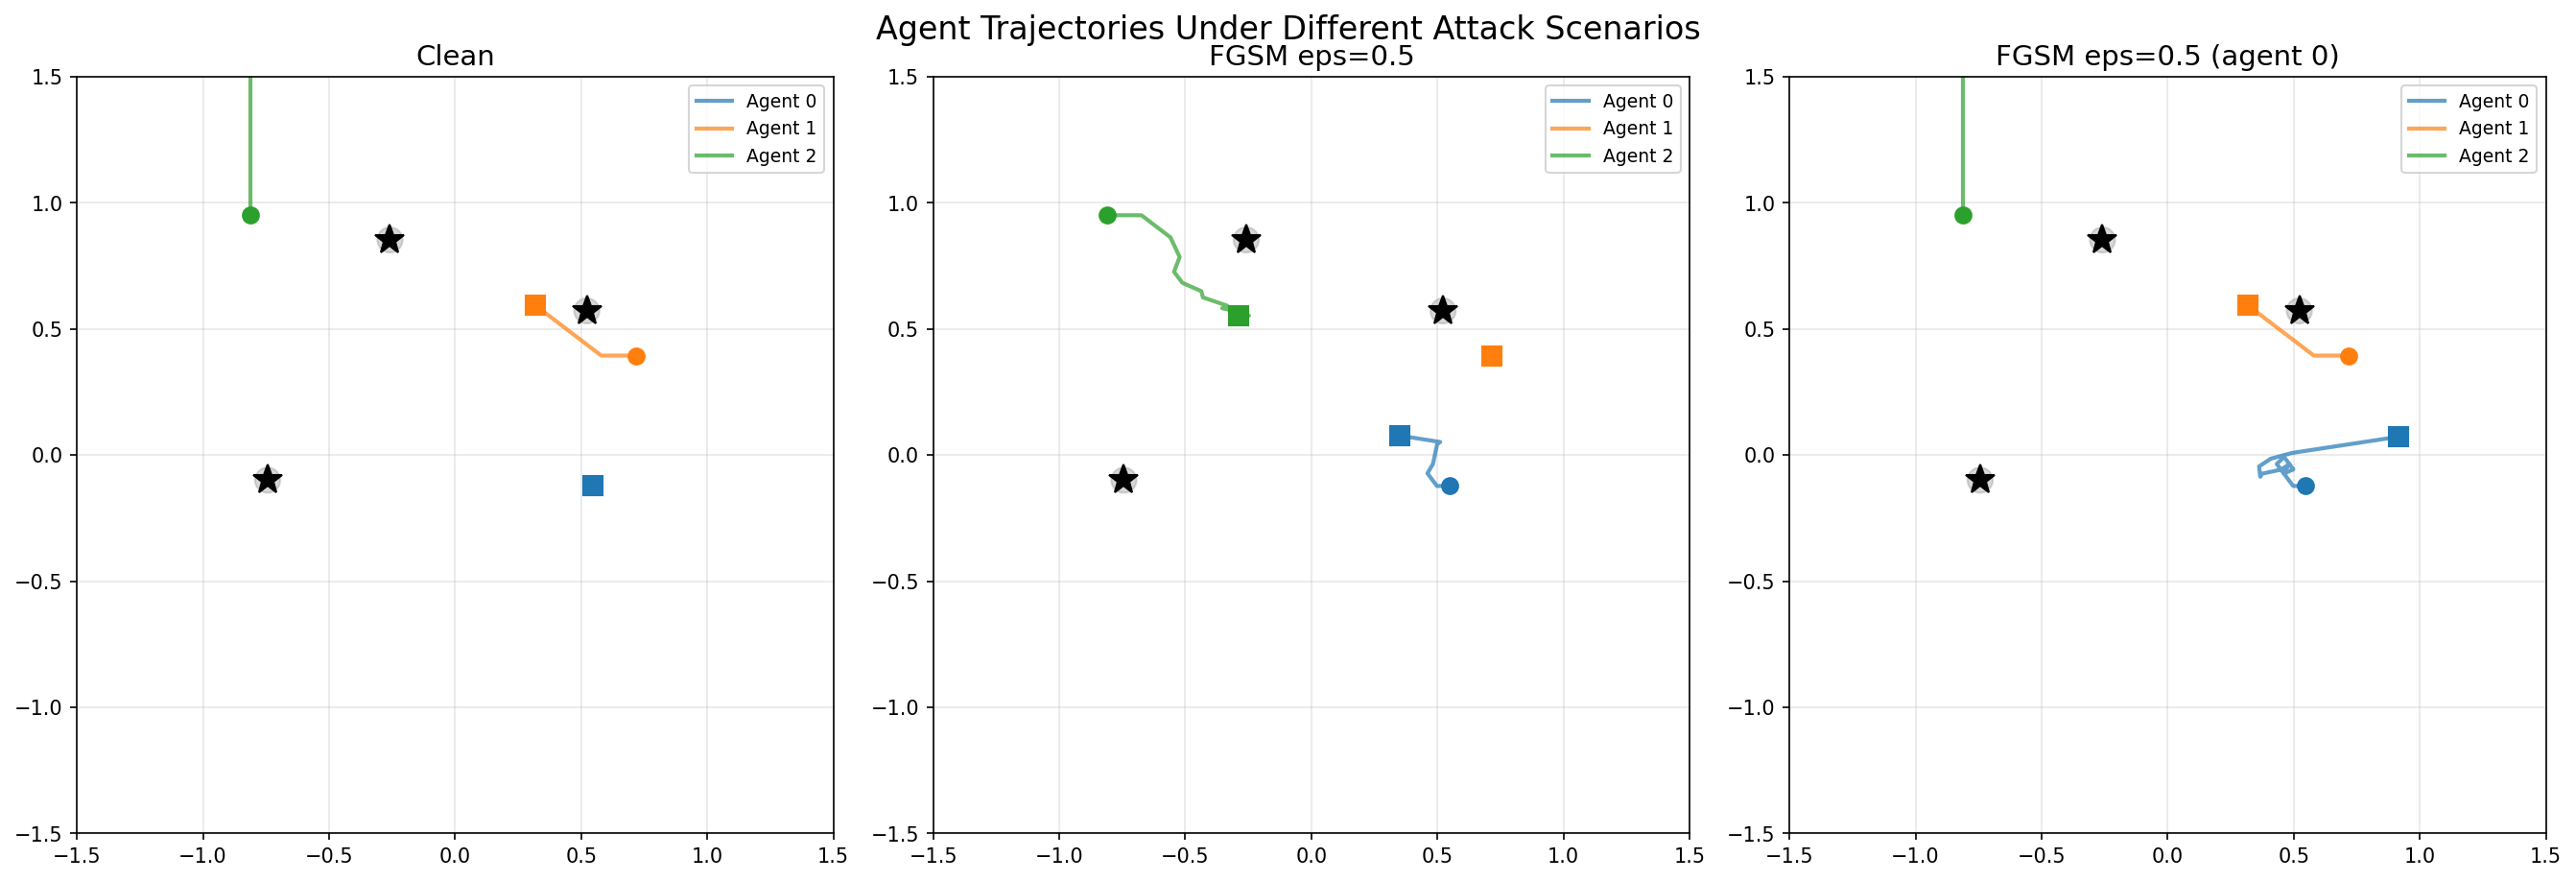
\includegraphics[width=\textwidth]{figures/trajectories.png}
\caption{Agent trajectories under different attack scenarios. Stars: landmarks. Circles: start positions. Squares: end positions. Under FGSM attack (middle), agents deviate from their clean trajectories. Attacking only agent~0 (right) causes localized disruption.}
\label{fig:trajectories}
\end{figure}

\subsection{Cross-Algorithm Transferability}
\label{sec:transferability}

\begin{table}[H]
\centering
\caption{Attack transferability between MAPPO and QMIX. ``Source'' indicates which model was used to craft the attack; ``Target'' indicates which model is attacked.}
\label{tab:transfer}
\begin{tabular}{llrr}
\toprule
Attack & Source $\to$ Target & Mean Reward & $\Delta$ vs.\ Clean \\
\midrule
Clean & MAPPO & $-68.3$ & --- \\
Clean & QMIX & $-167.0$ & --- \\
\midrule
FGSM ($\epsilon{=}0.5$) & MAPPO $\to$ MAPPO & $-73.0$ & $-7.0\%$ \\
FGSM ($\epsilon{=}0.5$) & MAPPO $\to$ QMIX & $-161.5$ & $+3.3\%$ \\
\midrule
Adversarial agent & MAPPO $\to$ MAPPO & $-97.2$ & $-42.3\%$ \\
Adversarial agent & MAPPO $\to$ QMIX & $-174.8$ & $-4.7\%$ \\
\bottomrule
\end{tabular}
\end{table}

\Cref{tab:transfer} shows limited transferability. FGSM perturbations crafted against MAPPO actually \emph{improve} QMIX's performance ($+3.3\%$), likely because the perturbation directions are policy-specific and may coincidentally push QMIX's observations toward better regions. The adversarial agent trained against MAPPO has modest impact on QMIX ($-4.7\%$) compared to its devastating effect on MAPPO ($-42.3\%$). This suggests that adversarial agents learn to exploit algorithm-specific cooperative strategies rather than universal vulnerabilities.

Note that QMIX's substantially worse clean performance ($-167.0$ vs.\ $-68.3$) is due to the challenge of training value decomposition methods on this task, which is consistent with prior benchmarking studies \citep{papoudakis2021benchmarking}.

\subsection{Communication Robustness}
\label{sec:comm_results}

\begin{figure}[H]
\centering
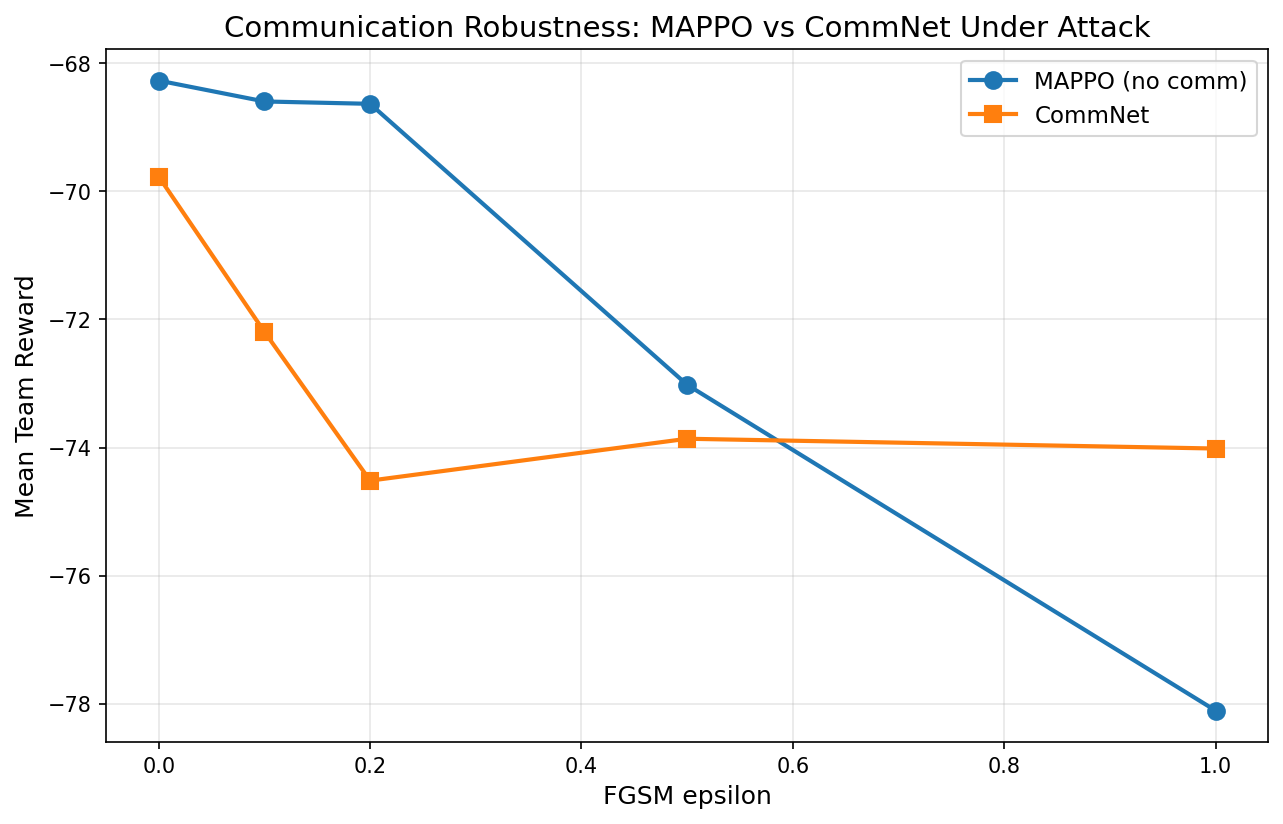
\includegraphics[width=0.8\textwidth]{figures/comm_robustness.png}
\caption{Robustness comparison between MAPPO (no communication) and CommNet under FGSM attack. CommNet is more vulnerable at low $\epsilon$ but more resilient at high $\epsilon$.}
\label{fig:comm_robustness}
\end{figure}

\begin{table}[H]
\centering
\caption{Communication robustness: relative reward degradation under FGSM attack.}
\label{tab:comm}
\begin{tabular}{lrr}
\toprule
FGSM $\epsilon$ & MAPPO degradation & CommNet degradation \\
\midrule
0.1 & $-0.5\%$ & $-3.5\%$ \\
0.2 & $-0.5\%$ & $-6.8\%$ \\
0.5 & $-7.0\%$ & $-5.9\%$ \\
1.0 & $-14.4\%$ & $-6.1\%$ \\
\bottomrule
\end{tabular}
\end{table}

\Cref{fig:comm_robustness,tab:comm} reveal a nuanced picture. At small perturbations ($\epsilon \leq 0.2$), CommNet is \emph{more vulnerable} than MAPPO: a small perturbation to one agent's observation propagates through the communication channel and affects all agents' decisions. However, at large perturbations ($\epsilon \geq 0.5$), CommNet plateaus while MAPPO continues to degrade. This suggests that at high noise levels, the communication messages from unperturbed agents provide a corrective signal that partially counteracts the adversarial noise. This finding has important implications for system design: communication is a double-edged sword in adversarial settings.

\subsection{Stealth Attack Trade-off}
\label{sec:stealth_results}

\begin{figure}[H]
\centering
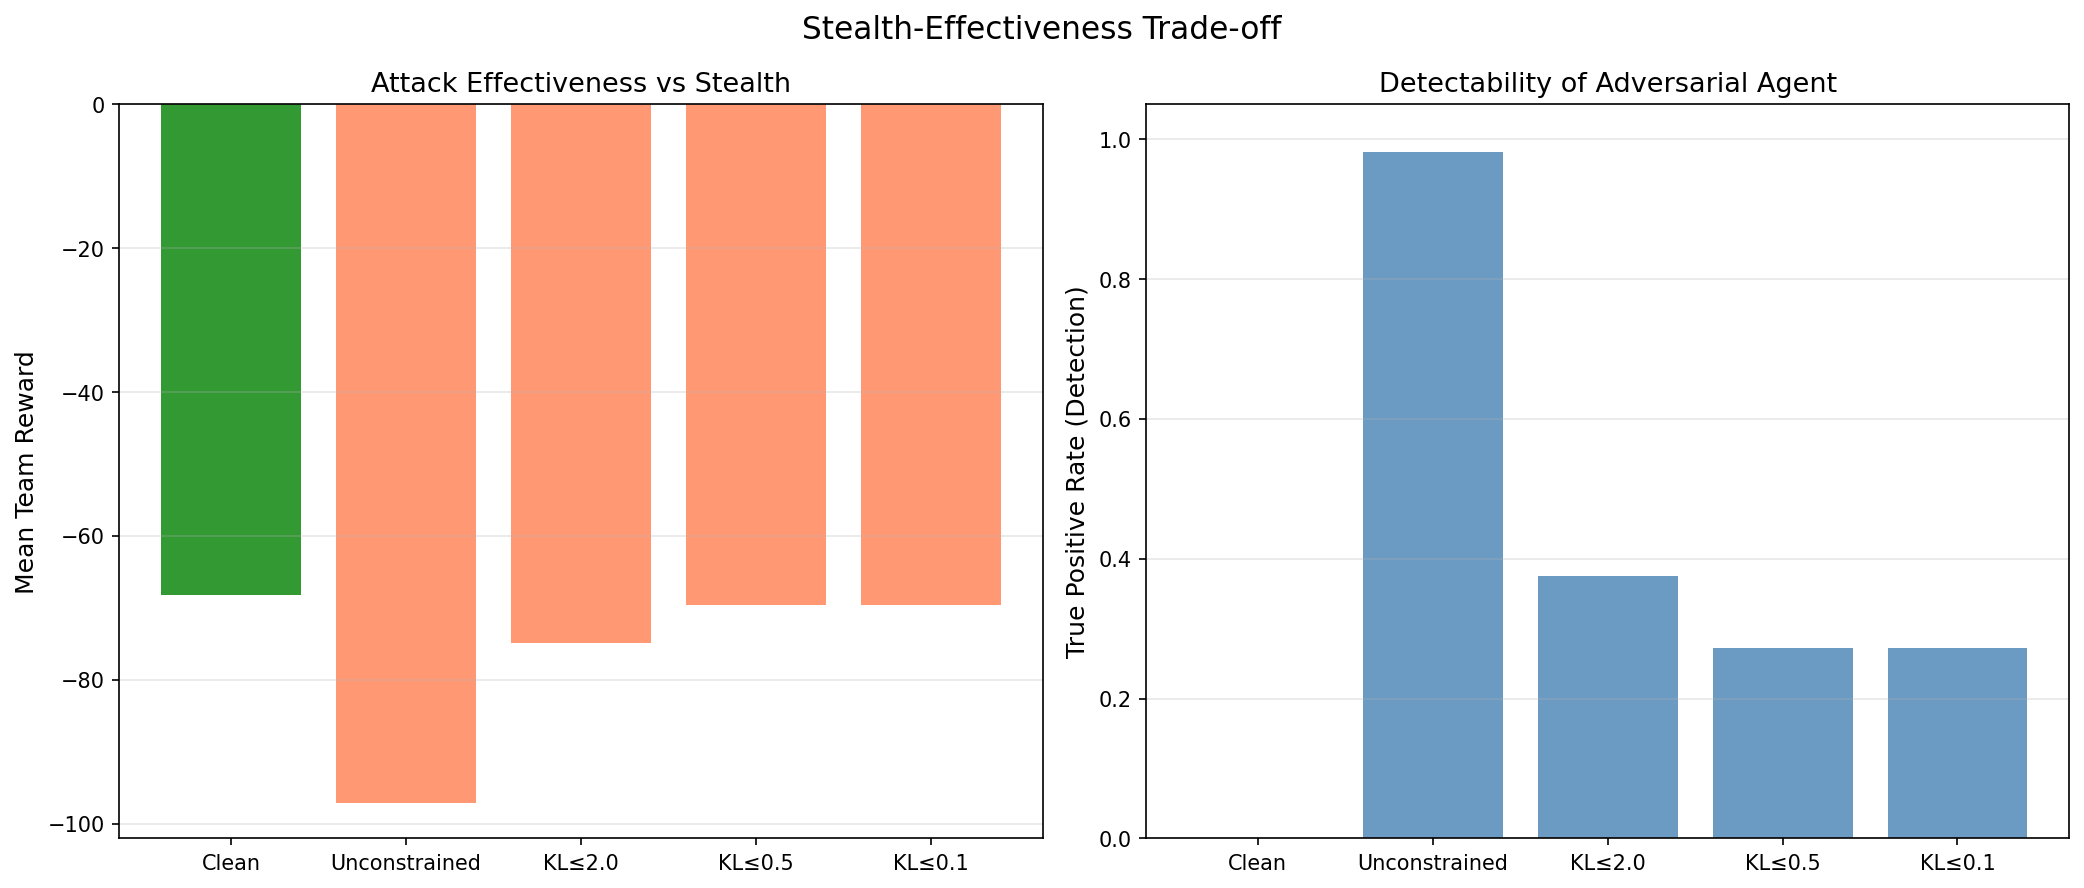
\includegraphics[width=\textwidth]{figures/stealth_tradeoff.png}
\caption{Left: attack effectiveness (lower reward = more effective attack). Right: detectability (TPR of anomaly detector). The unconstrained adversary is highly effective but easily detected. Stealth agents sacrifice effectiveness for undetectability.}
\label{fig:stealth}
\end{figure}

\begin{table}[H]
\centering
\caption{Stealth attack trade-off: effectiveness vs.\ detectability.}
\label{tab:stealth}
\begin{tabular}{lrrr}
\toprule
Agent type & Mean Reward & $\Delta$ vs.\ Clean & TPR (\%) \\
\midrule
Clean & $-68.3$ & --- & $0.0$ \\
Unconstrained adversary & $-97.2$ & $-42.3\%$ & $98.2$ \\
Stealth ($\delta = 2.0$) & $-74.9$ & $-9.7\%$ & $37.5$ \\
Stealth ($\delta = 0.5$) & $-69.7$ & $-2.0\%$ & $27.3$ \\
Stealth ($\delta = 0.1$) & $-69.7$ & $-2.0\%$ & $27.3$ \\
\bottomrule
\end{tabular}
\end{table}

\Cref{fig:stealth,tab:stealth} reveal a clear trade-off between attack effectiveness and stealth. The unconstrained adversary degrades team performance by 42.3\% but is detected 98.2\% of the time. The stealth adversary with $\delta = 2.0$ achieves a meaningful 9.7\% degradation while reducing the detection rate to 37.5\%. Tighter constraints ($\delta \leq 0.5$) yield adversaries with minimal impact ($-2.0\%$) and lower but non-trivial detection rates (27.3\% TPR). That $\delta = 0.1$ and $\delta = 0.5$ produce identical results suggests both constraints are tight enough that the adversary effectively converges to the cooperative policy---the constraint dominates the adversarial objective.

The false positive rate is 0\% across all experiments, indicating that the anomaly detector never falsely accuses cooperative agents. This asymmetry---high specificity, variable sensitivity---suggests that detection is reliable when it fires, but stealthy adversaries can operate under the detection threshold.

\subsection{Countermeasure Evaluation}

\begin{figure}[H]
\centering
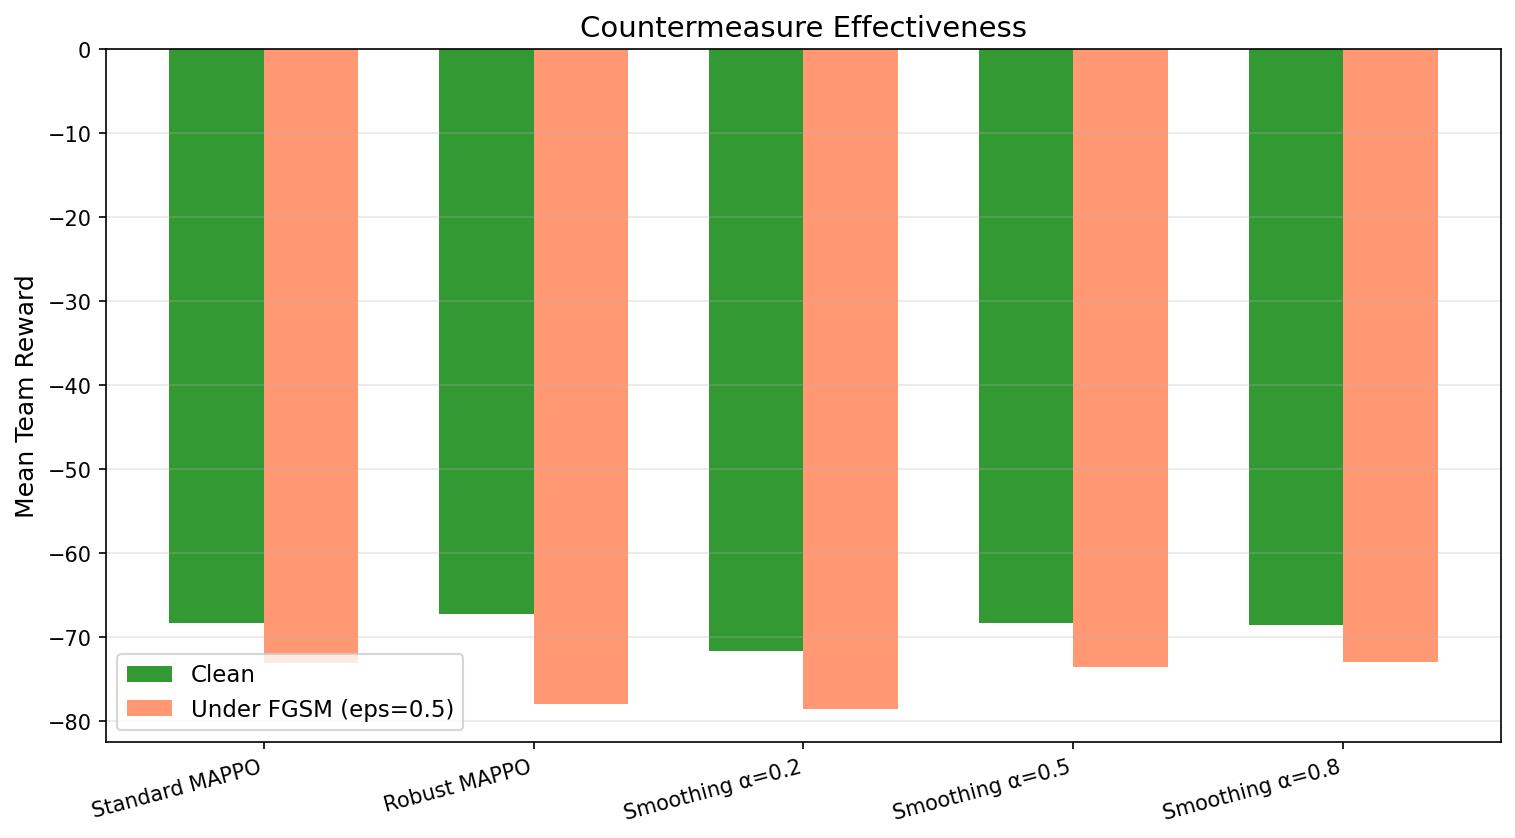
\includegraphics[width=0.9\textwidth]{figures/countermeasures.png}
\caption{Countermeasure effectiveness. Green: clean performance. Orange: under FGSM ($\epsilon = 0.5$).}
\label{fig:countermeasures}
\end{figure}

\begin{table}[H]
\centering
\caption{Countermeasure evaluation against FGSM ($\epsilon = 0.5$), 5 training seeds with 95\% CIs. Adaptive attack compensates for smoothing attenuation by scaling $\epsilon$ by $1/\alpha$.}
\label{tab:counter}
\begin{tabular}{lrr}
\toprule
Defense & Clean [95\% CI] & FGSM [95\% CI] \\
\midrule
Standard MAPPO & $-65.5\ [-69.9, -61.1]$ & $-75.0\ [-79.6, -70.3]$ \\
FGSM adv.\ training & $-95.2\ [-105, -85]$ & $-102\ [-112, -91]$ \\
Smoothing $\alpha = 0.5$ & $-65.9\ [-70.8, -61.0]$ & $-75.6\ [-80.0, -71.1]$ \\
Smoothing $\alpha = 0.8$ & $-65.4\ [-69.9, -61.0]$ & $-75.3\ [-78.7, -71.8]$ \\
\midrule
\multicolumn{3}{l}{\textit{Adaptive attack (FGSM scaled through smoother):}} \\
Smoothing $\alpha = 0.5$ & --- & $-85.4\ [-90.4, -80.4]$ \\
Smoothing $\alpha = 0.8$ & --- & $-77.3\ [-81.6, -72.9]$ \\
\bottomrule
\end{tabular}
\end{table}

\Cref{fig:countermeasures,tab:counter} present several findings.

\textbf{FGSM adversarial training destabilizes learning.} Training with FGSM perturbations during data collection severely degrades clean performance ($-95.2$ vs.\ $-65.5$), making the policy worse than random agents ($-77$). The FGSM perturbations likely corrupt the advantage estimates and policy gradient signal, preventing convergence. This contrasts with supervised learning, where adversarial training is effective, and highlights a challenge specific to on-policy RL.

\textbf{Observation smoothing provides marginal benefit under standard attack} ($-75.3$ vs.\ $-75.0$ for $\alpha = 0.8$), and the CIs overlap substantially. Under an \emph{adaptive} attacker who compensates for the smoothing attenuation by scaling $\epsilon$ by $1/\alpha$, the defense provides no meaningful improvement ($-77.3$). This demonstrates the importance of evaluating defenses against adaptive adversaries \citep{madry2018towards}.

\textbf{No tested defense substantially reduces FGSM vulnerability} at $\epsilon = 0.5$. This motivates future work on certified defenses or architecture-level robustness.

% ═════════════════════════════════════════════════════════════════════
% CHAPTER 7: DISCUSSION
% ═════════════════════════════════════════════════════════════════════
\section{Discussion}
\label{sec:discussion}

\subsection{Behavioral vs.\ Observation Attacks}

Our results show that behavioral attacks (adversarial agent replacement) are far more devastating than observation perturbation attacks: $-42.3\%$ vs.\ $-14.4\%$ for the strongest FGSM. However, this comparison must be interpreted with care, because the two attack types operate under fundamentally different threat models. Observation perturbation assumes the attacker can add bounded noise to sensor readings---a realistic threat in many settings. Adversarial agent replacement assumes the attacker has \emph{full insider access}: the ability to replace an agent's entire policy with a malicious one, which requires compromising the agent's software or hardware. The asymmetry in attacker power naturally leads to asymmetry in attack effectiveness.

The practical implication is not simply that ``behavioral attacks are worse,'' but rather that \emph{the two threats require different defenses}: observation perturbation calls for robust perception (smoothing, certified defenses), while agent compromise calls for access control, attestation, and anomaly detection.

\subsection{The Communication Paradox}

Our finding that communication increases vulnerability at low perturbation levels is both novel and practically significant. The mechanism is intuitive: in CommNet, each agent's message is a function of its (potentially corrupted) observation. When one agent receives adversarial input, its message carries adversarial information to all other agents, effectively amplifying the attack.

However, at high noise levels, the averaging operation in CommNet acts as a low-pass filter: the mean of $n-1$ clean messages and 1 corrupted message dilutes the adversarial signal. This creates a robustness floor that MAPPO (without such averaging) lacks.

Practical recommendation: communication protocols in adversarial environments should incorporate message validation or robust aggregation (e.g., median instead of mean) to mitigate propagation of adversarial noise.

\subsection{Stealth and the Detectability Frontier}

The stealth attack experiments reveal a fundamental tension in adversarial MARL. An effective adversary must deviate from cooperative behavior, but deviation enables detection. The KL constraint provides a principled way to navigate this trade-off. Importantly, the detection rate never drops to zero---even stealth adversaries exhibit subtle statistical signatures. This suggests that sufficiently sensitive detectors could, in principle, identify all adversarial agents, albeit at the cost of increased false positive rates (which we did not observe due to our conservative threshold).

\subsection{Transferability Implications}

Our transferability results are \emph{exploratory} and must be interpreted cautiously due to the QMIX convergence gap. The limited transfer we observe could reflect genuine algorithmic specificity---MAPPO's policy gradient landscape differs fundamentally from QMIX's value decomposition---but it could also reflect the poor quality of the QMIX target policy. Prior work has demonstrated transferability of adversarial examples in cooperative MARL within the same algorithm family \citep{guo2022towards}; our results suggest that cross-family transfer may be weaker, but confirming this requires matched baselines. We test only MAPPO~$\to$~QMIX, not the reverse direction.

\subsection{Limitations}

This work has several limitations:

\begin{enumerate}
    \item \textbf{Environment scope.} We evaluate on Simple Spread, a relatively simple environment. Results may not generalize to more complex tasks (e.g., StarCraft~II) with richer dynamics and larger agent populations.

    \item \textbf{QMIX convergence.} Our QMIX implementation did not fully converge (clean reward $-167$ vs.\ MAPPO's $-68$), making transferability comparisons difficult to interpret in absolute terms.

    \item \textbf{Attack budget.} We evaluate only inference-time attacks. Training-time attacks (e.g., reward poisoning, data poisoning) may be more effective and are left for future work.

    \item \textbf{Training seed variance.} We train with five independent seeds and report confidence intervals for key results, but additional seeds would strengthen the statistical claims further.

    \item \textbf{Stealth constraint.} The KL divergence is computed globally rather than conditioned on specific states, which may allow state-specific deviations that are harder to detect.
\end{enumerate}

\subsection{Ethical Considerations}

This work studies attacks on cooperative AI systems. While our intent is to understand vulnerabilities and develop defenses, the techniques could potentially be misused. We emphasize that all experiments are conducted in simulated environments for research purposes. The countermeasures we evaluate provide actionable defense strategies for practitioners deploying cooperative MARL systems.

% ═════════════════════════════════════════════════════════════════════
% CHAPTER 8: CONCLUSION
% ═════════════════════════════════════════════════════════════════════
\section{Conclusion}
\label{sec:conclusion}

This thesis presents a systematic study of adversarial attacks on cooperative multi-agent reinforcement learning systems. We evaluate observation perturbation attacks (FGSM, PGD) and behavioral attacks (adversarial agent replacement) against three cooperative algorithms (MAPPO, QMIX, CommNet) and investigate three novel research questions: stealth attacks, cross-algorithm transferability, and communication robustness.

Our key findings are:

\begin{enumerate}
    \item \textbf{Behavioral attacks are far more effective, but under a stronger threat model.} A trained adversarial agent degrades team performance by 42\%, compared to 25\% for the strongest observation perturbation ($p < 0.01$). However, the two attacks assume fundamentally different attacker capabilities (sensor noise vs.\ insider compromise), and require different defensive strategies.

    \item \textbf{FGSM outperforms PGD in discrete action spaces.} Single-step attacks cross more decision boundaries than iterative attacks. This finding is robust across a PGD ablation (3--50 steps, with/without random start) and is specific to discrete-action policies.

    \item \textbf{Cross-algorithm transferability appears limited (exploratory).} Attacks crafted against MAPPO do not effectively transfer to QMIX, though QMIX convergence limitations temper this conclusion.

    \item \textbf{Communication is a double-edged sword.} CommNet amplifies adversarial noise at low perturbation levels but provides resilience at high levels through message averaging.

    \item \textbf{Stealth attacks reveal a clear effectiveness--detectability trade-off.} KL-constrained adversaries at $\delta = 2.0$ achieve 10\% reward degradation with reduced detection (TPR $= 37.5\%$), while tighter constraints ($\delta \leq 0.5$) effectively prevent adversarial behavior.

    \item \textbf{No tested defense substantially mitigates FGSM.} FGSM adversarial training destabilizes RL, observation smoothing provides only marginal benefit, and adaptive attackers can compensate for smoothing. This motivates future work on certified defenses.
\end{enumerate}

\subsection{Future Work}

Several promising directions extend this work:

\begin{itemize}
    \item Evaluating on more complex environments (SMAC, Multi-Agent MuJoCo) with larger agent populations and continuous action spaces.
    \item Investigating training-time attacks, including reward poisoning and gradient manipulation during centralized training.
    \item Developing communication-aware defenses, such as robust message aggregation and Byzantine-tolerant communication protocols.
    \item Exploring state-conditional stealth constraints that allow the adversary to deviate more in low-information states.
    \item Combining multiple countermeasures (smoothing + detection + adversarial training) for layered defense.
\end{itemize}

% ═════════════════════════════════════════════════════════════════════
% BIBLIOGRAPHY
% ═════════════════════════════════════════════════════════════════════
\bibliographystyle{plainnat}
\bibliography{references}

\end{document}
